% !Mode:: "TeX:DE:UTF-8:Main"

\documentclass[aspectratio=169]{beamer}
\usepackage[svgnames,x11names]{xcolor}
\usepackage{tikzlings}

\setbeamertemplate{navigation symbols}{}
\setbeamertemplate{background canvas}{%
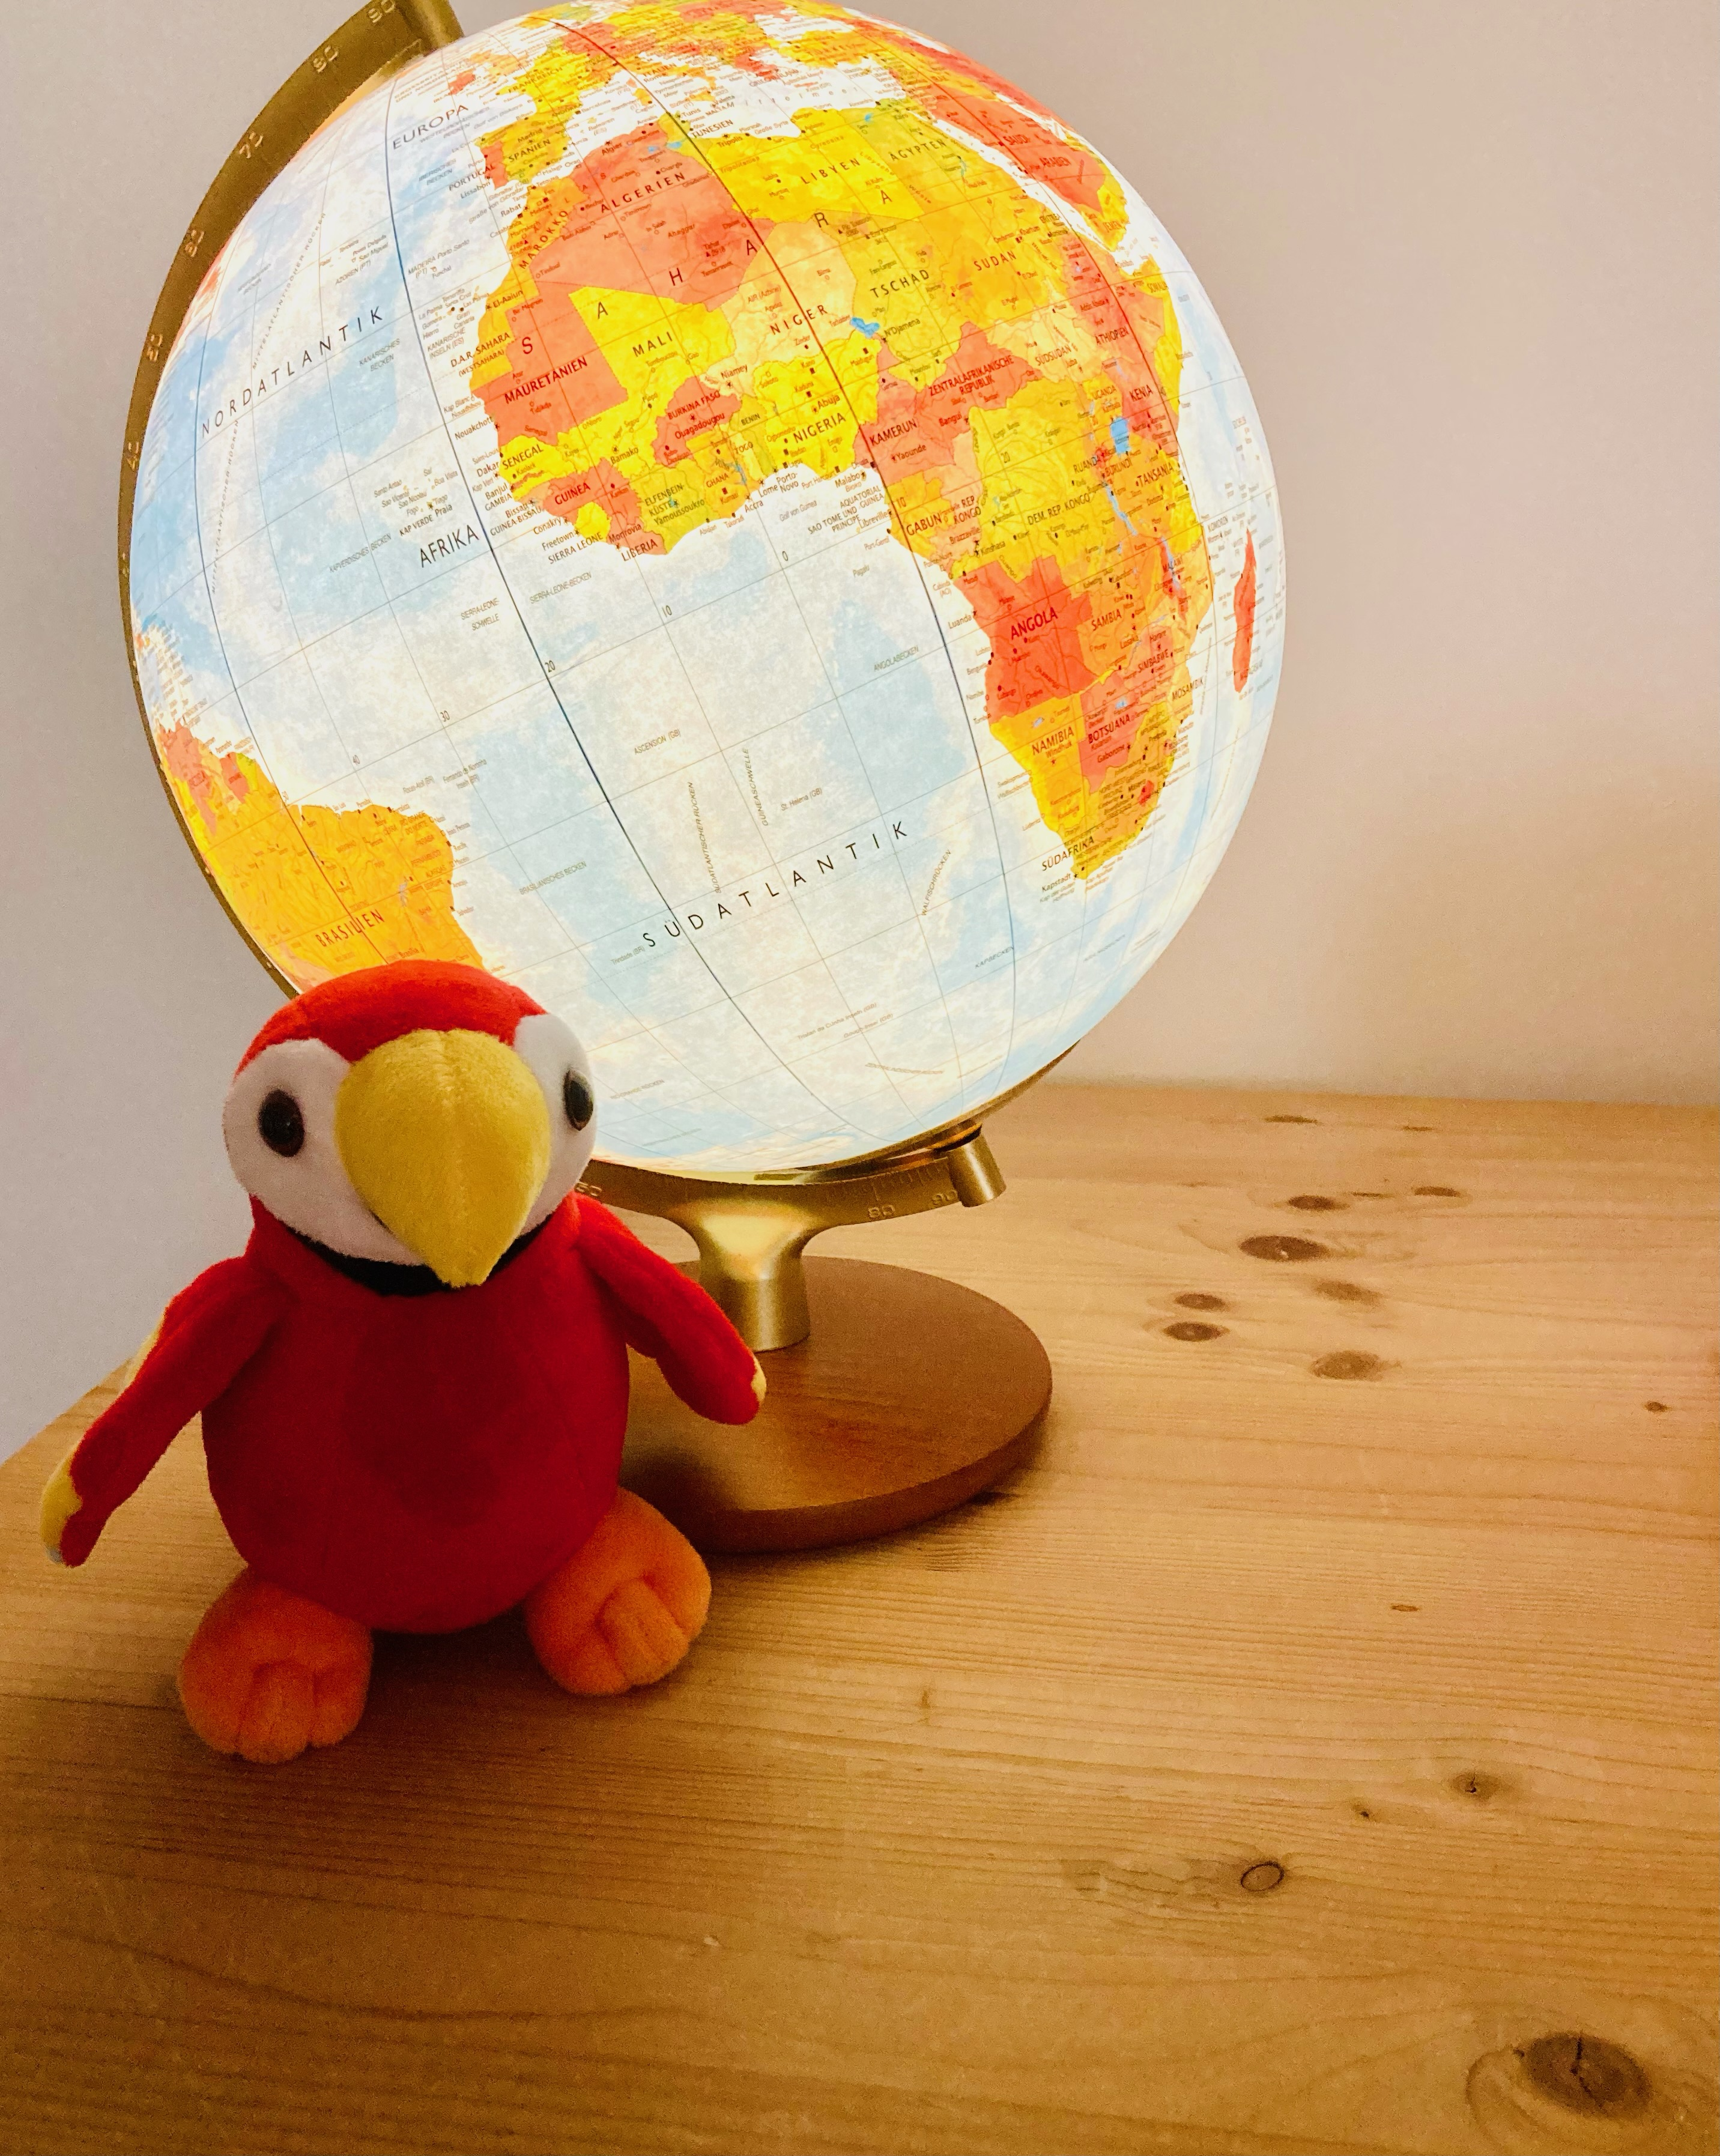
\includegraphics[trim=0cm 10cm 0cm 0cm,width=\paperwidth,height=\paperheight,keepaspectratio]{joyoftheworld}%
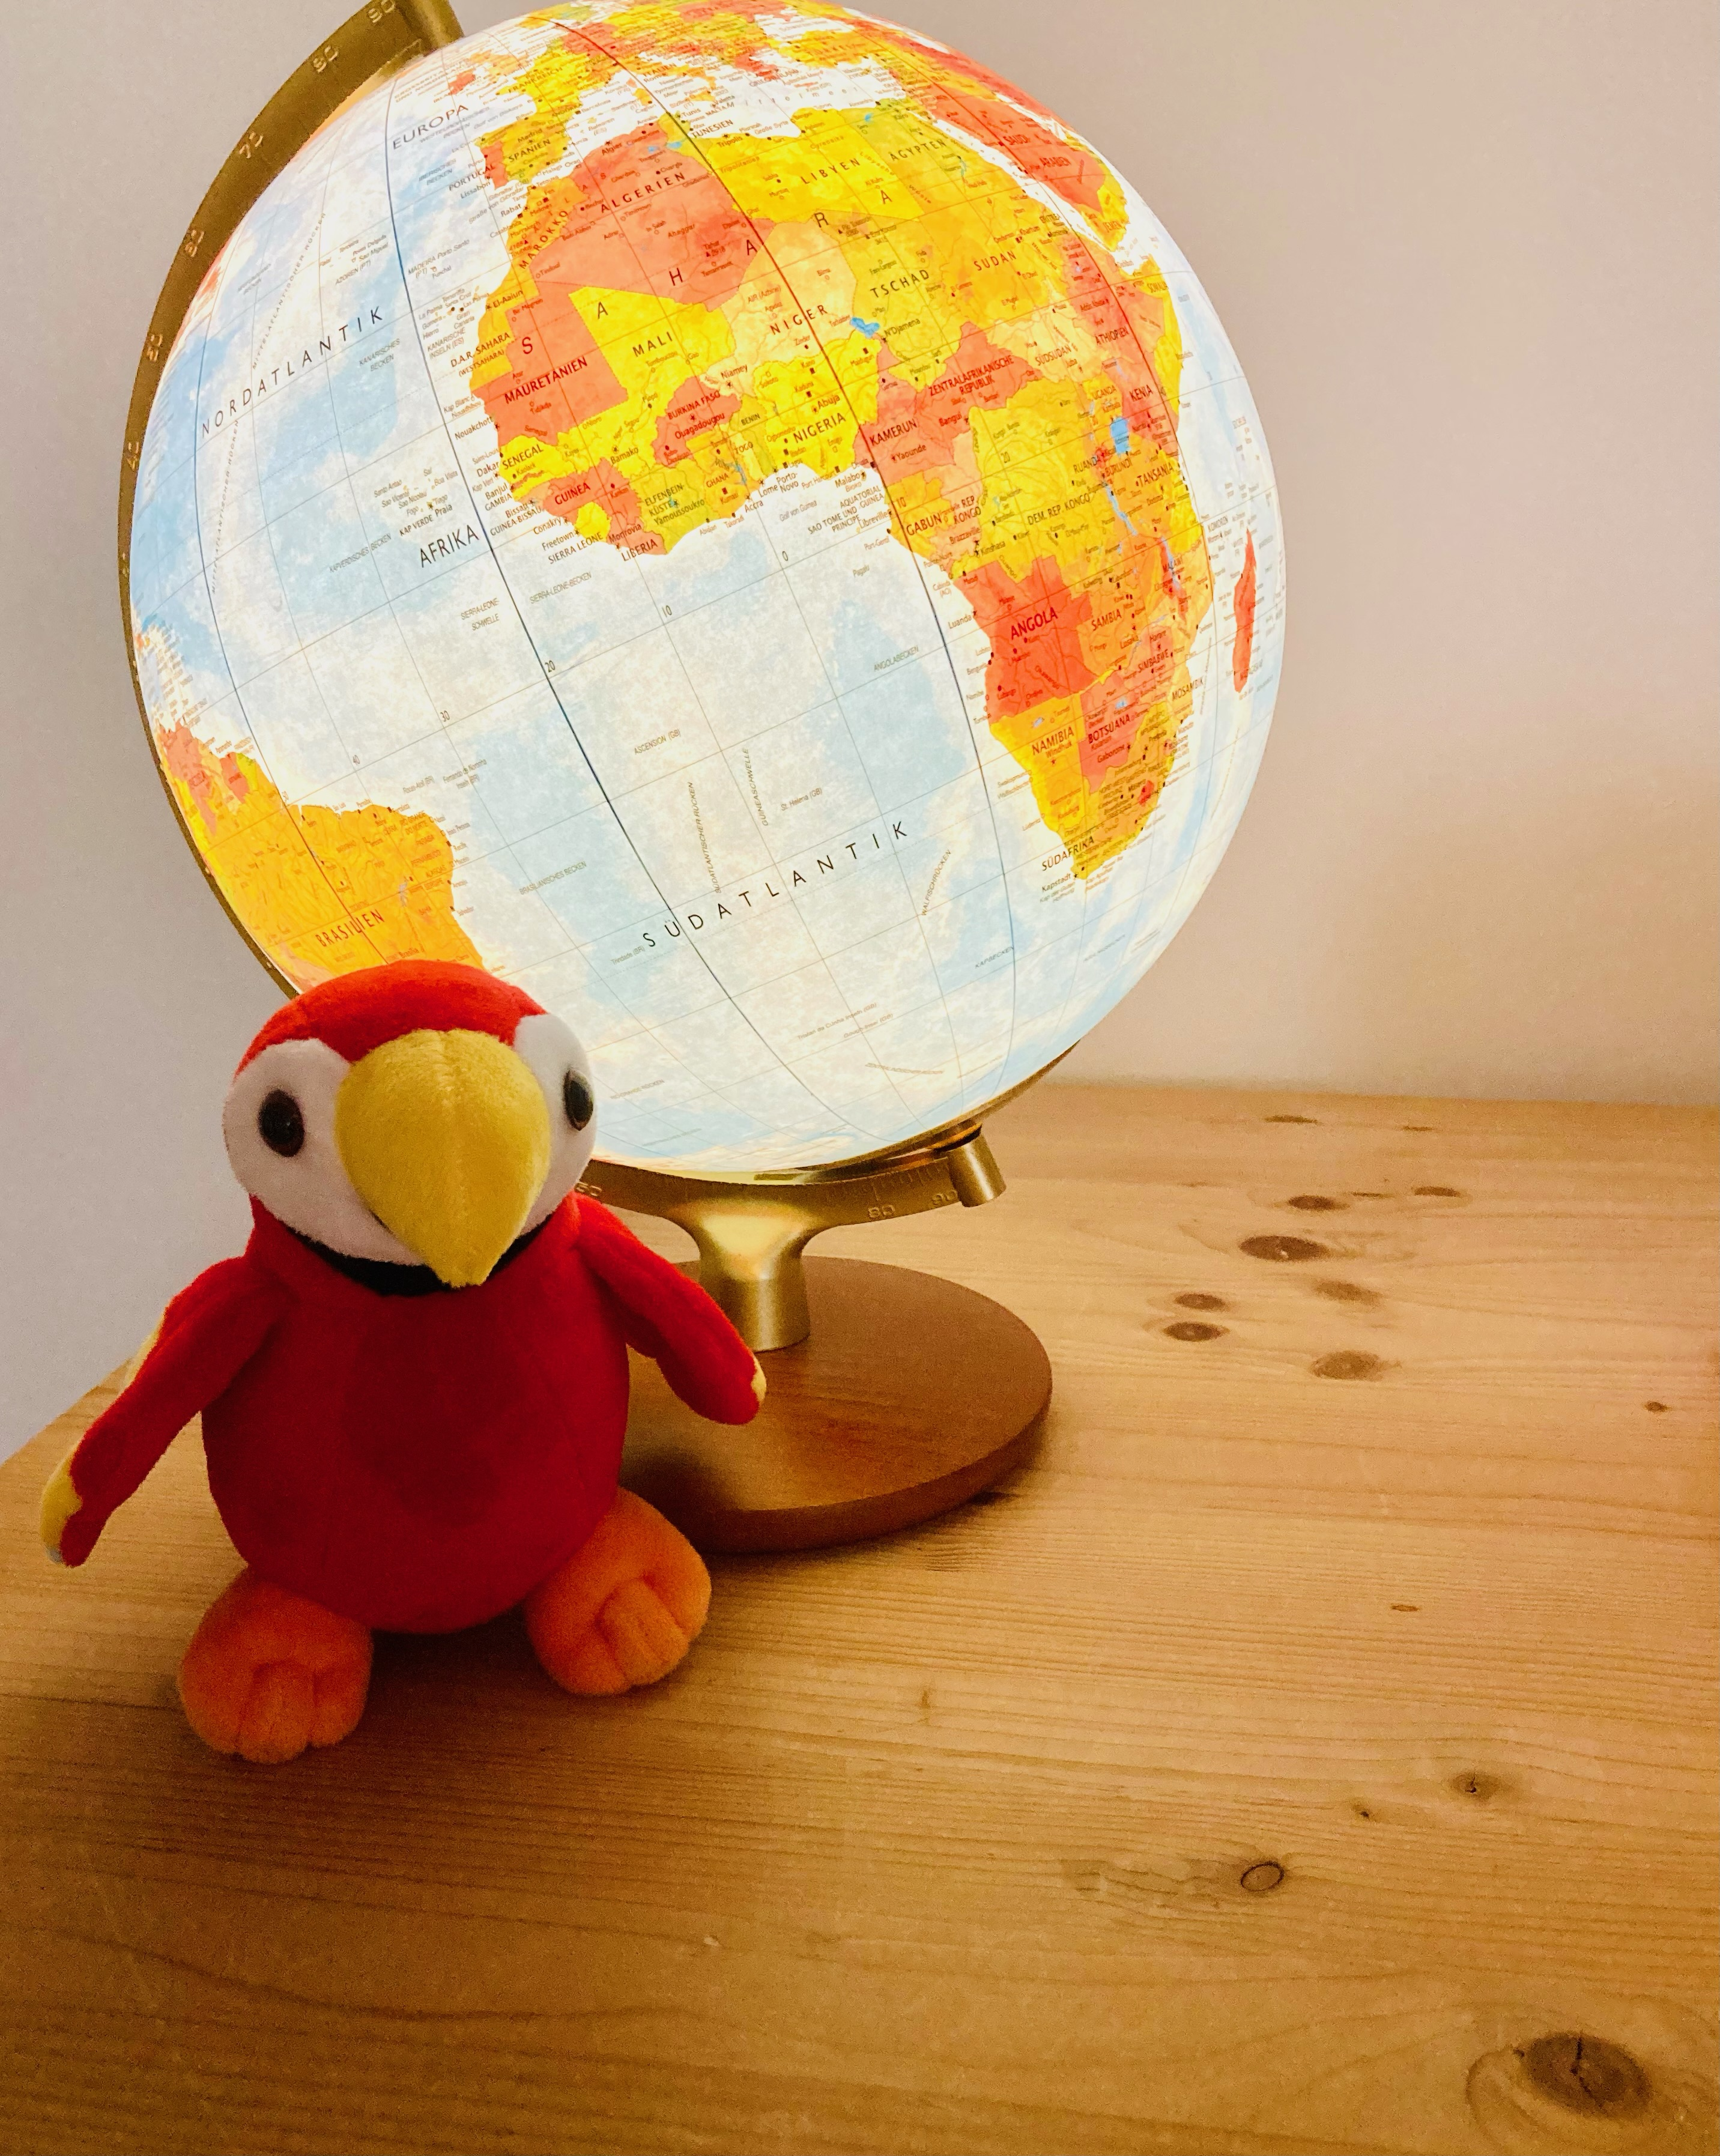
\includegraphics[clip,trim=75cm 10cm 0cm 0cm,width=\paperwidth,height=\paperheight,keepaspectratio]{joyoftheworld}%
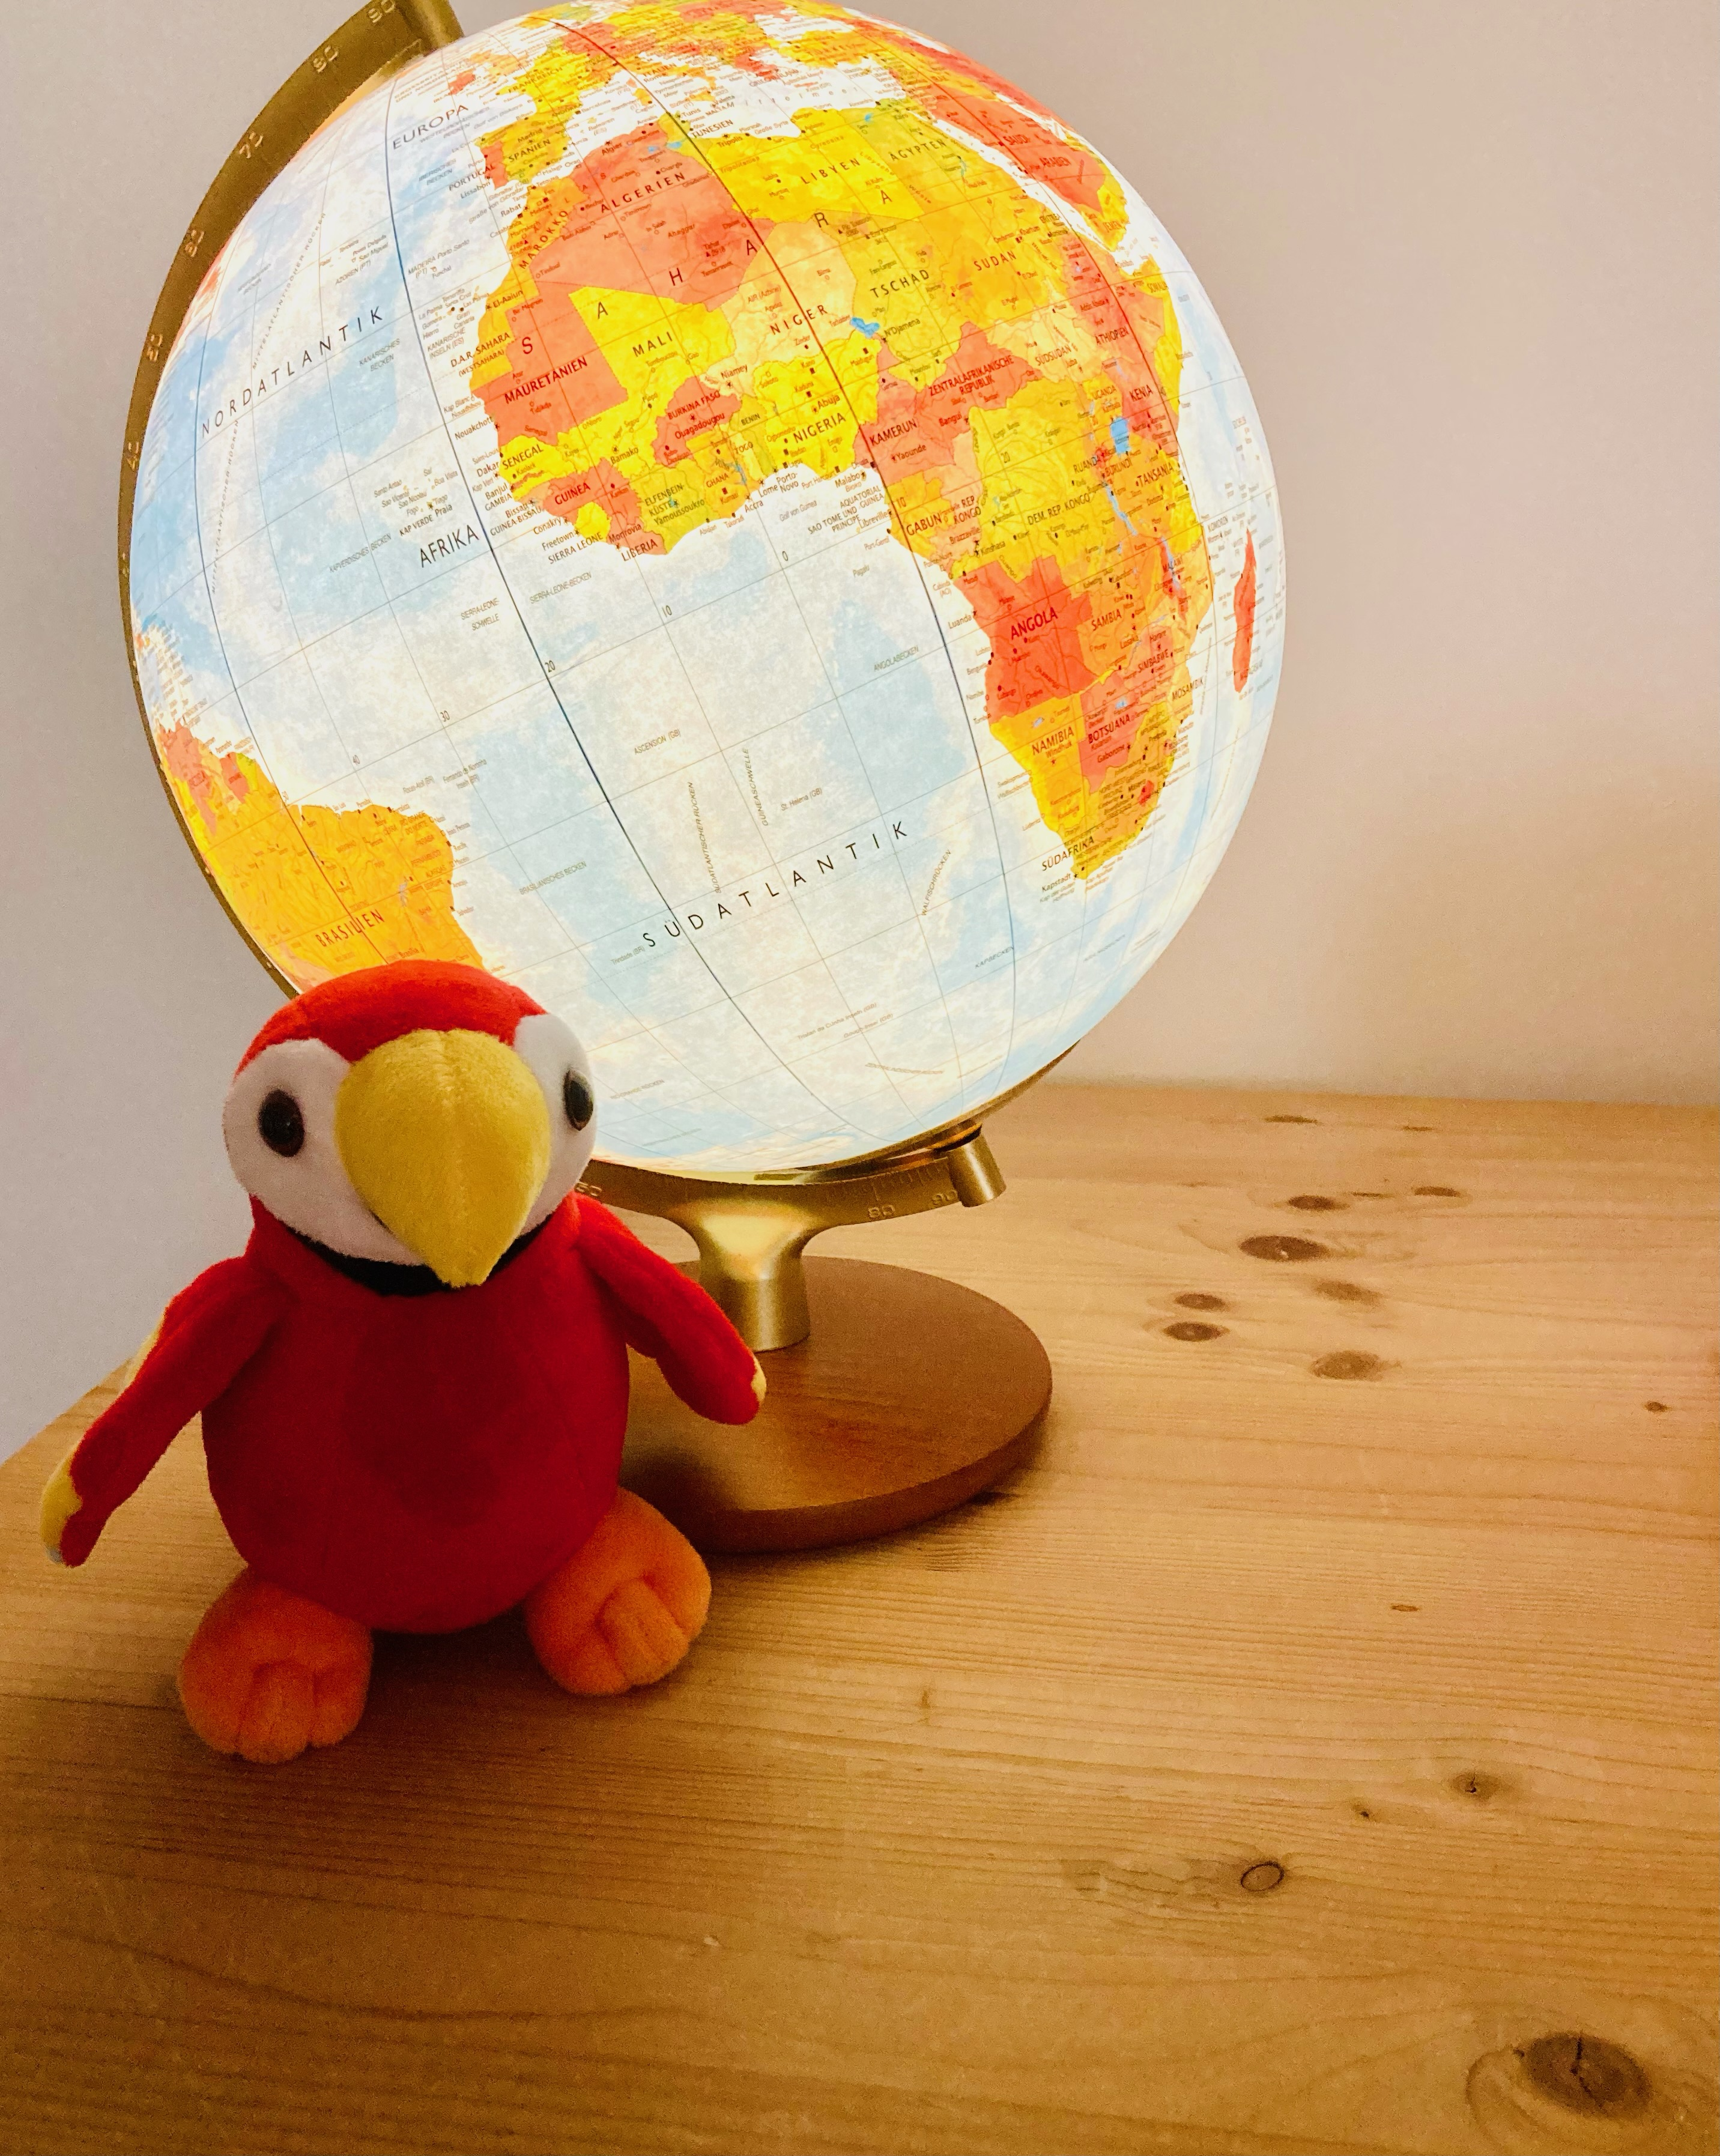
\includegraphics[clip,trim=75cm 10cm 0cm 0cm,width=\paperwidth,height=\paperheight,keepaspectratio]{joyoftheworld}%
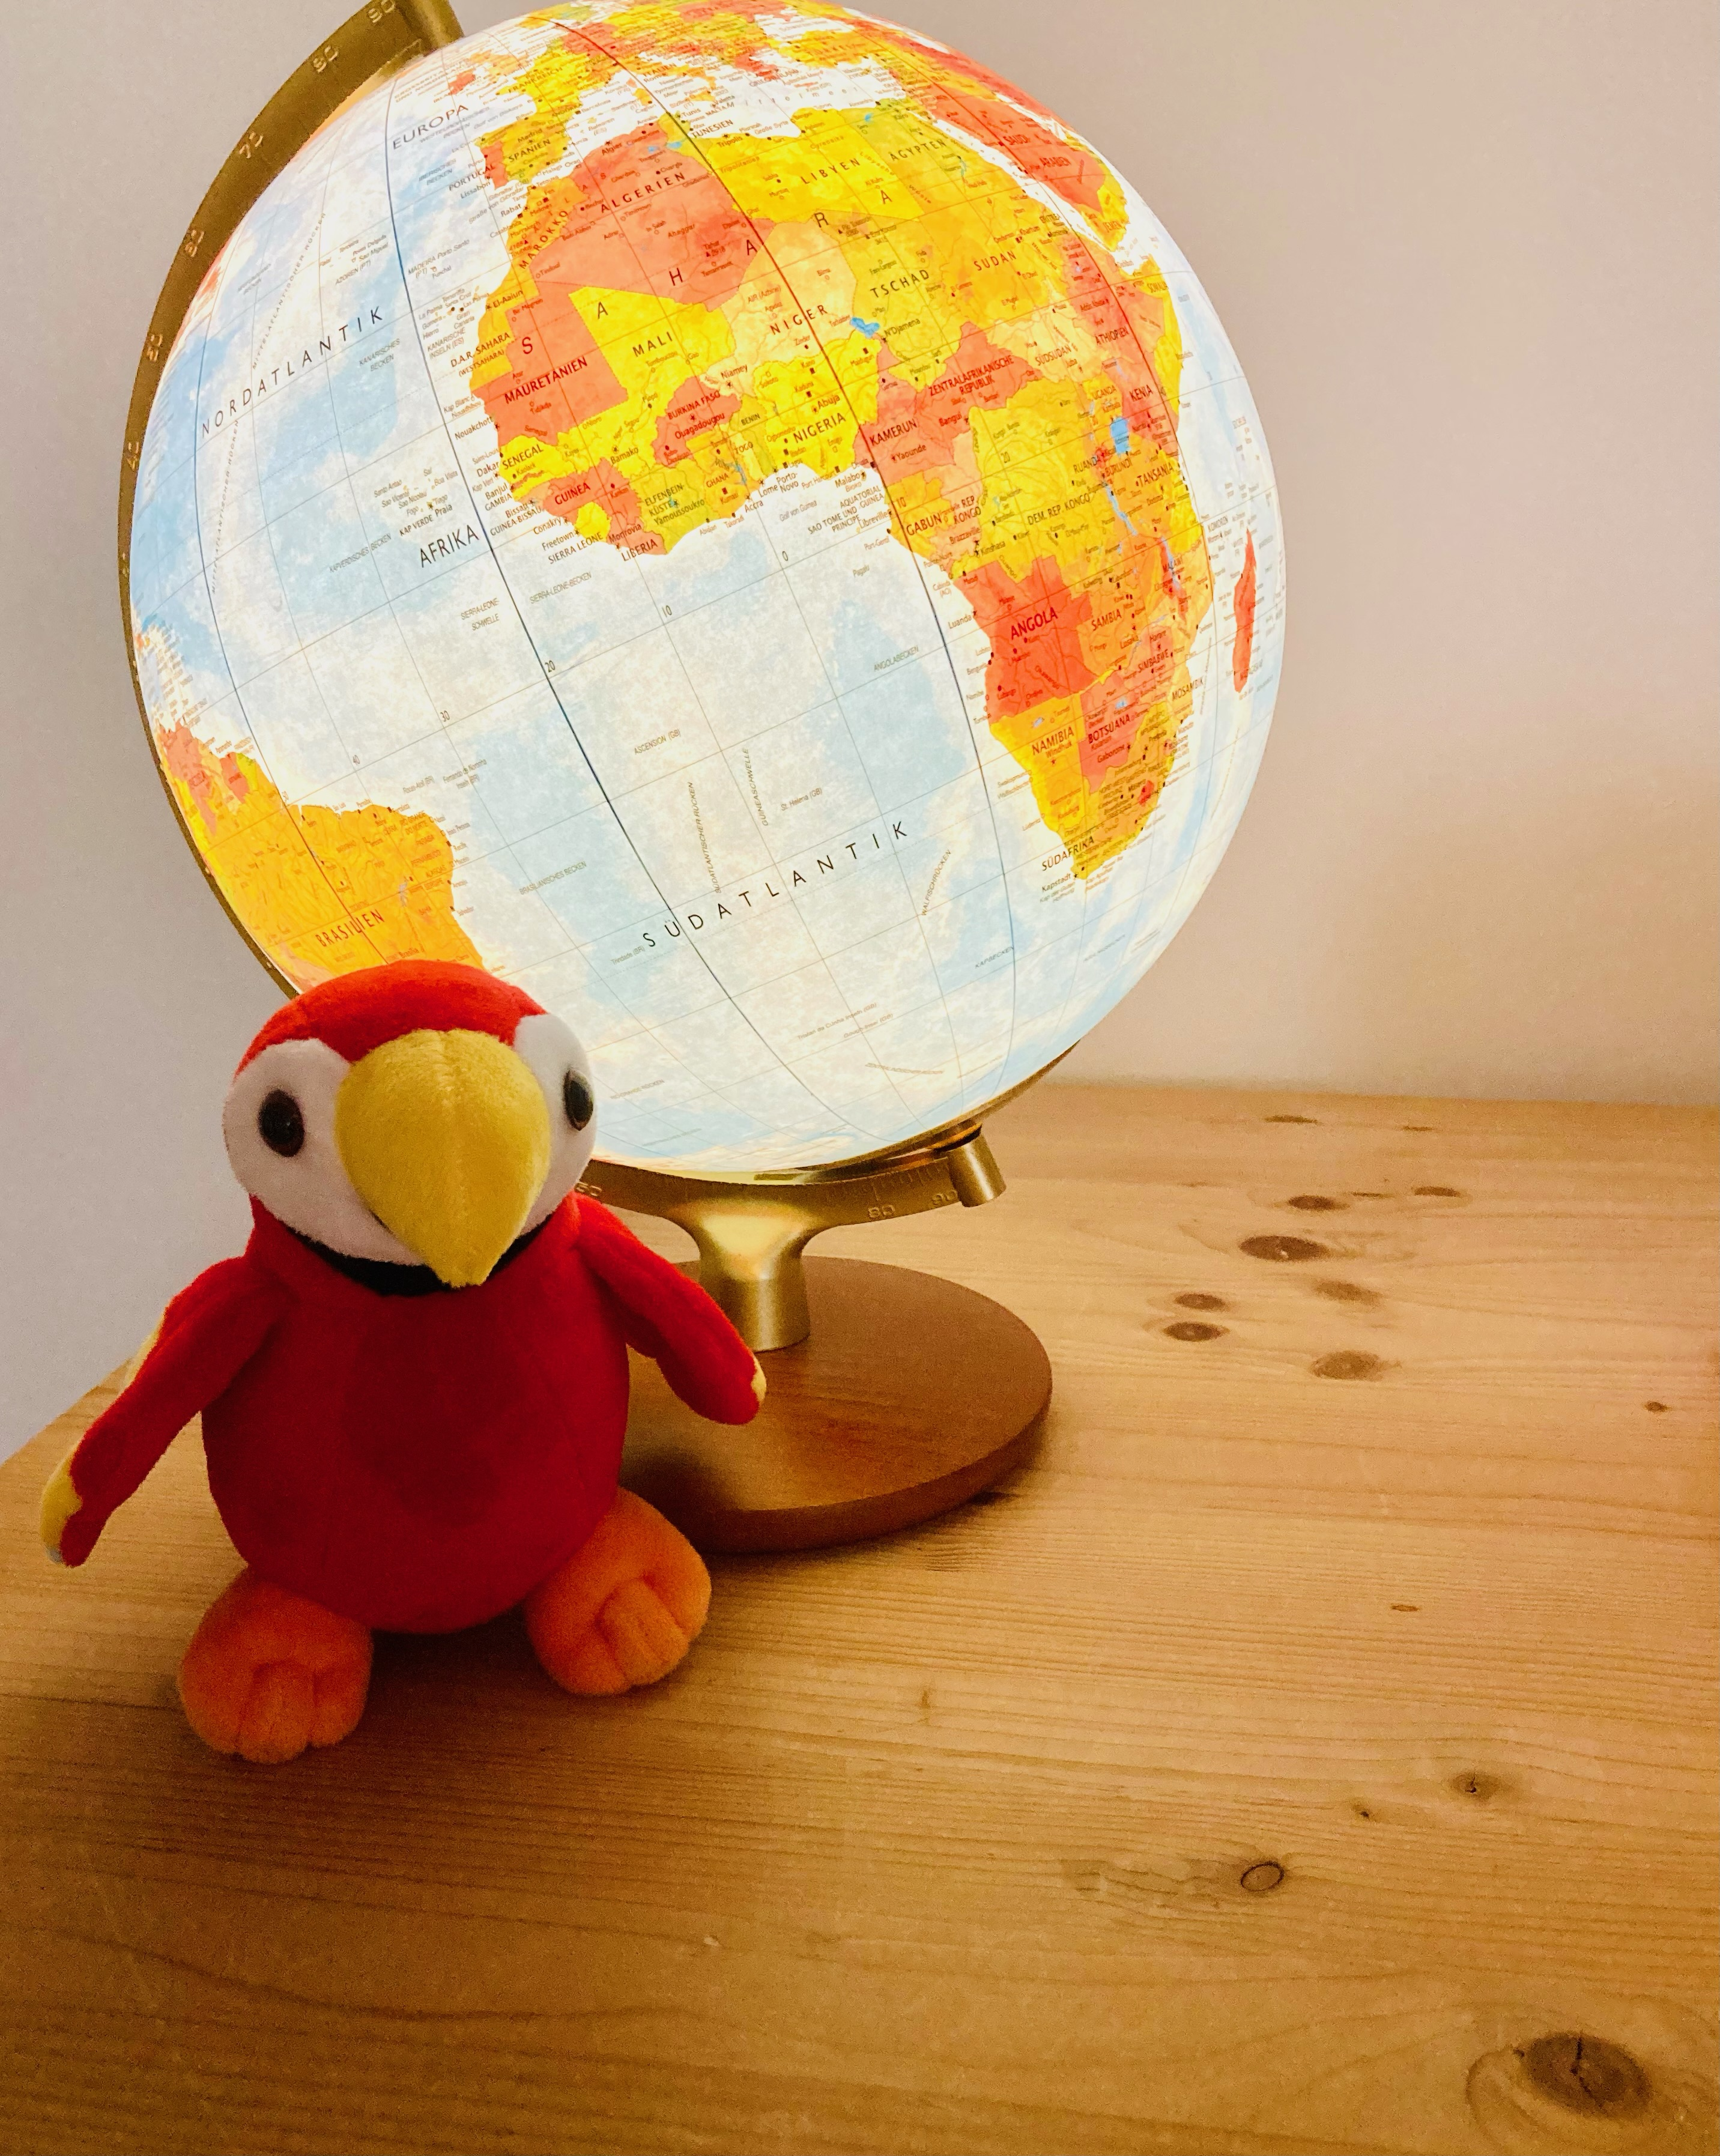
\includegraphics[clip,trim=75cm 10cm 0cm 0cm,width=\paperwidth,height=\paperheight,keepaspectratio]{joyoftheworld}%
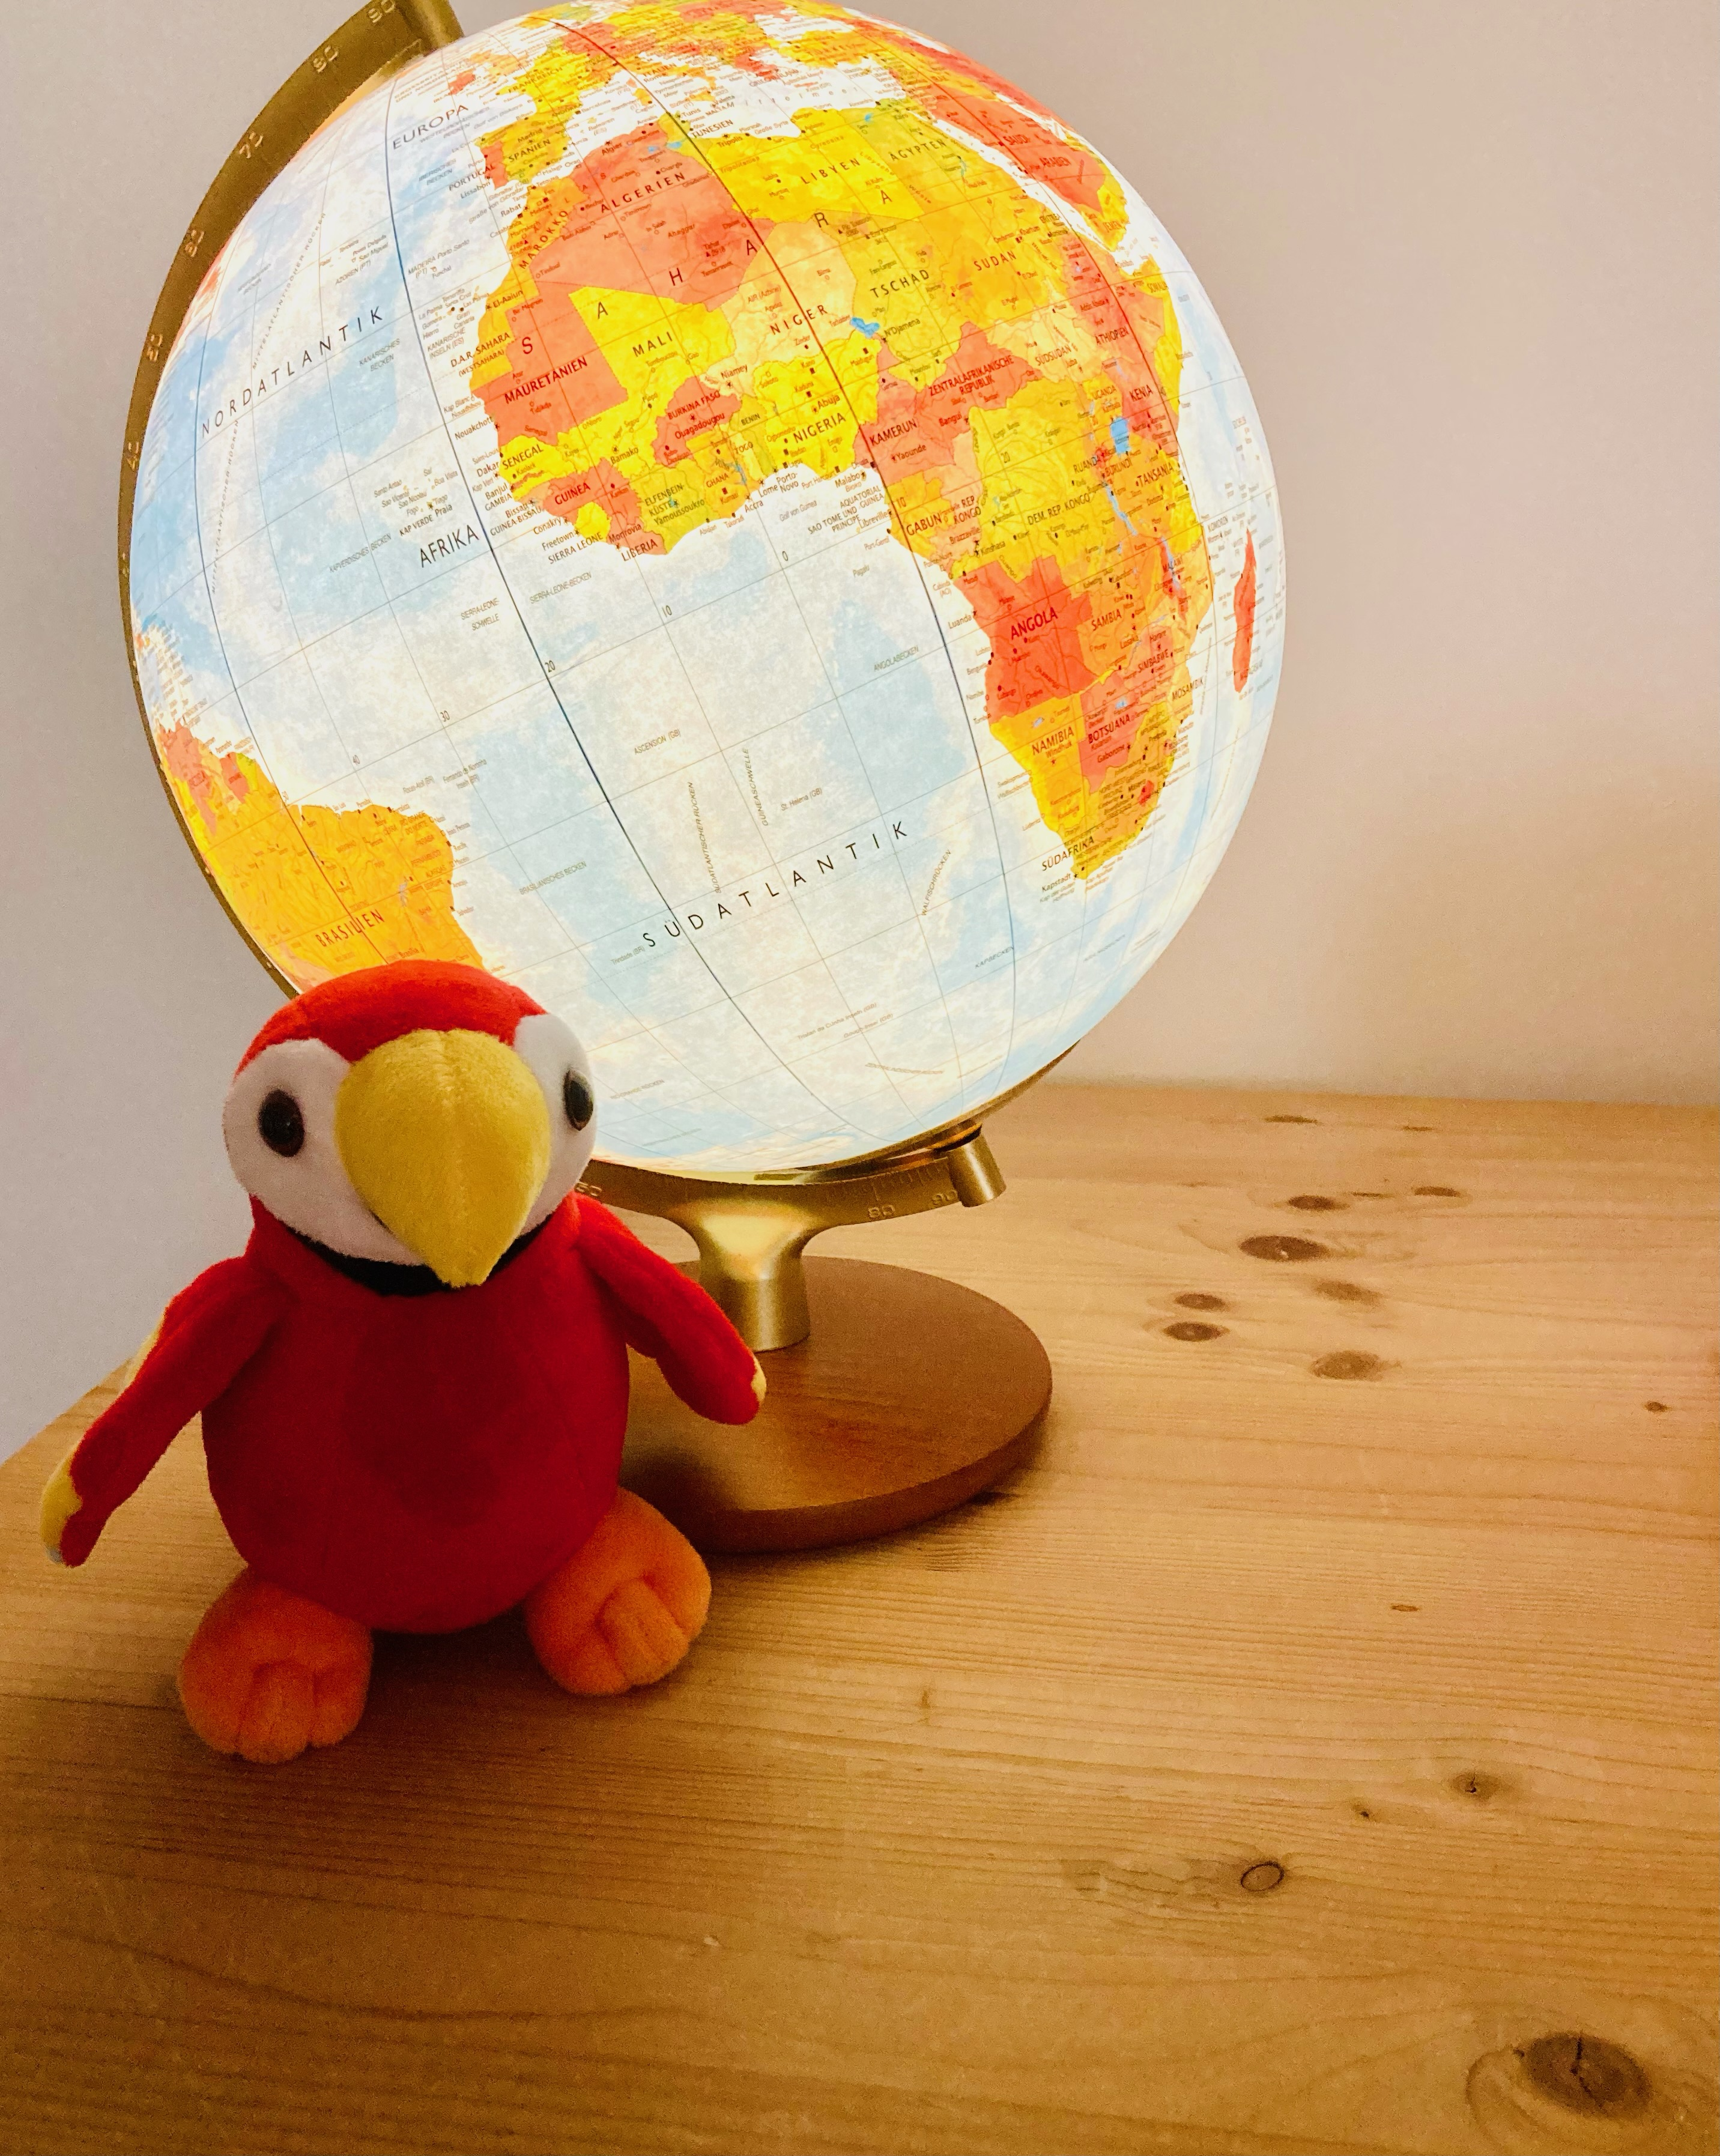
\includegraphics[clip,trim=75cm 10cm 0cm 0cm,width=\paperwidth,height=\paperheight,keepaspectratio]{joyoftheworld}%
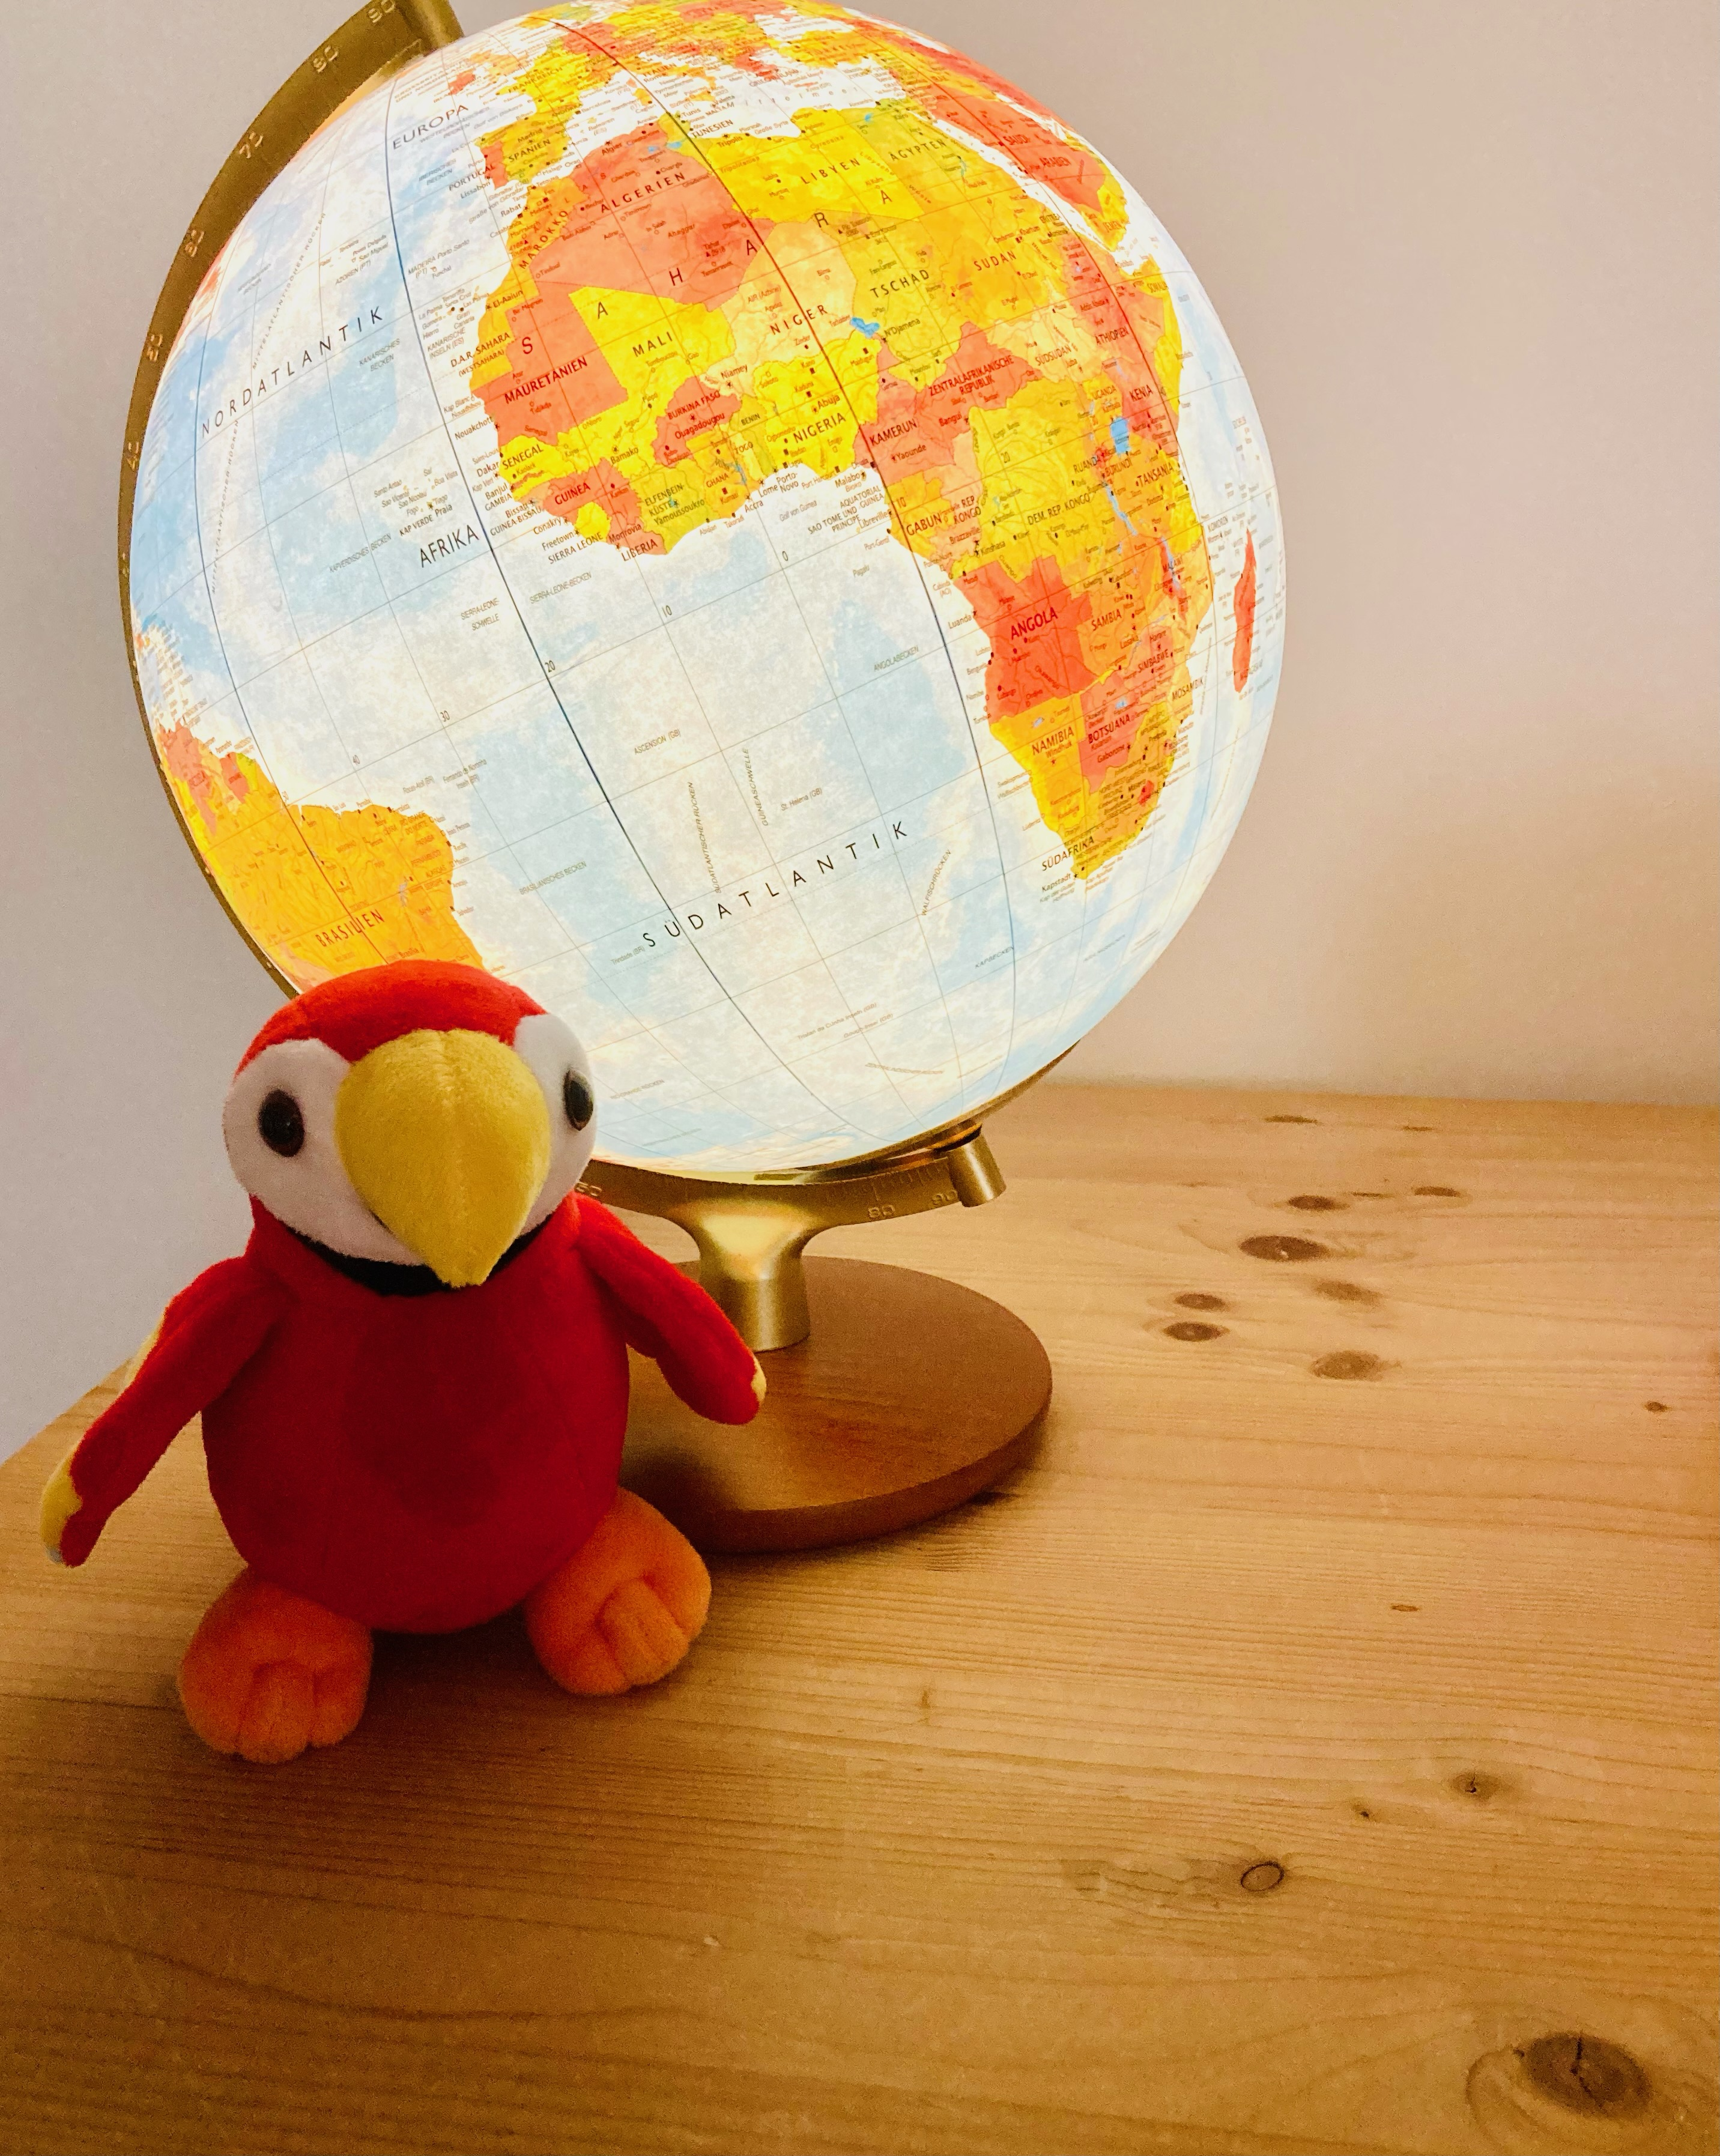
\includegraphics[clip,trim=75cm 10cm 0cm 0cm,width=\paperwidth,height=\paperheight,keepaspectratio]{joyoftheworld}%
}
\graphicspath{{include/}}

% trick taken from https://topanswers.xyz/tex?q=1989
\tikzset{
    use page relative coordinates/.style={
        shift={(current page.south west)},
        x={(current page.south east)},
        y={(current page.north west)}
    },
}

\ExplSyntaxOn
\let\intmodnn\int_mod:nn
\ExplSyntaxOff
\tikzset{invclip/.style={clip,insert path={{[reset cm]
      (-16383.99999pt,-16383.99999pt) rectangle (16383.99999pt,16383.99999pt)
    }}}}
\begin{document}
	
\begin{frame}
  \begin{tikzpicture}[remember picture, overlay]
 \begin{scope}[even odd rule] 
 \path[invclip] (4,4)-- (5,2) -- (5,-2) -- (2,-4) -- (0,-5)--(-5,-6)--(-5,6)--cycle;   
 %\fill[Goldenrod](-6,-7) rectangle (15,7);
 \end{scope} 
    \node at (6.65,1) {
		\ifnum \intmodnn{\thepage}{6} > 2
			
\includegraphics[width=3cm]{mouse_close}%
		\else
			
\includegraphics[width=3cm]{mouse_open}%
		\fi%
	};	 
   	\node at (9,1.5) {
		\ifnum \intmodnn{\thepage}{6} > 2
			
\includegraphics[width=3cm]{mouse_close}%
		\else
			
\includegraphics[width=3cm]{mouse_open}%
		\fi%
	};	
	\node at (13.5,2) {
		\ifnum \intmodnn{\thepage}{6} > 3
			
\includegraphics[width=3cm]{mouse_close}%
		\else
			
\includegraphics[width=3cm]{mouse_open}%
		\fi%
	};
	\node at (11.35,1) {
		\ifnum \intmodnn{\thepage}{6} > 2
			
\includegraphics[width=3cm]{mouse_close}%
		\else
			
\includegraphics[width=3cm]{mouse_open}%
		\fi%
	};			  
   \node at (6.65,-0.5) {
		\ifnum \intmodnn{\thepage}{6} > 2
			
\includegraphics[width=3cm]{mouse_close}%
		\else
			
\includegraphics[width=3cm]{mouse_open}%
		\fi%
	};	  
   	\node at (9,0) {
		\ifnum \intmodnn{\thepage}{6} > 2
			
\includegraphics[width=3cm]{mouse_close}%
		\else
			
\includegraphics[width=3cm]{mouse_open}%
		\fi%
	};	
	\node at (13.5,0.5) {
		\ifnum \intmodnn{\thepage}{6} > 3
			
\includegraphics[width=3cm]{mouse_close}%
		\else
			
\includegraphics[width=3cm]{mouse_open}%
		\fi%
	};
	\node at (11.35,-0.5) {
		\ifnum \intmodnn{\thepage}{6} > 2
			
\includegraphics[width=3cm]{mouse_close}%
		\else
			
\includegraphics[width=3cm]{mouse_open}%
		\fi%
	};
	\node at (6.65,-2) {
		\ifnum \intmodnn{\thepage}{6} > 2
			
\includegraphics[width=3cm]{mouse_close}%
		\else
			
\includegraphics[width=3cm]{mouse_open}%
		\fi%
	};	
		  
   	\node at (9,-1.5) {
		\ifnum \intmodnn{\thepage}{6} > 2
			
\includegraphics[width=3cm]{mouse_close}%
		\else
			
\includegraphics[width=3cm]{mouse_open}%
		\fi%
	};	
	\node at (13.5,-1) {
		\ifnum \intmodnn{\thepage}{6} > 3
			
\includegraphics[width=3cm]{mouse_close}%
		\else
			
\includegraphics[width=3cm]{mouse_open}%
		\fi%
	};
	\node at (11.35,-2) {
		\ifnum \intmodnn{\thepage}{6} > 2
			
\includegraphics[width=3cm]{mouse_close}%
		\else
			
\includegraphics[width=3cm]{mouse_open}%
		\fi%
	};
   \node at (6.65,-3.5) {
		\ifnum \intmodnn{\thepage}{6} > 2
			
\includegraphics[width=3cm]{mouse_close}%
		\else
			
\includegraphics[width=3cm]{mouse_open}%
		\fi%
	};	
   	\node at (9,-3) {
		\ifnum \intmodnn{\thepage}{6} > 2
			
\includegraphics[width=3cm]{mouse_close}%
		\else
			
\includegraphics[width=3cm]{mouse_open}%
		\fi%
	};	
	\node at (13.5,-2.5) {
		\ifnum \intmodnn{\thepage}{6} > 3
			
\includegraphics[width=3cm]{mouse_close}%
		\else
			
\includegraphics[width=3cm]{mouse_open}%
		\fi%
	};
	\node at (11.35,-3.5) {
		\ifnum \intmodnn{\thepage}{6} > 2
			
\includegraphics[width=3cm]{mouse_close}%
		\else
			
\includegraphics[width=3cm]{mouse_open}%
		\fi%
	};

\thing[santa,yshift=0.1cm,xshift=5.95cm]
\thing[santa=yellow!60!brown!60!orange,yshift=0.6cm,xshift=8.3cm]
\thing[santa=blue!70!black,yshift=1.1cm,xshift=12.8cm]
\thing[santa,yshift=0.1cm,xshift=10.65cm]

\thing[santa,yshift=-1.4cm,xshift=5.95cm]
\thing[santa=yellow!60!brown!60!orange,yshift=-0.9cm,xshift=8.3cm]
\thing[santa=blue!70!black,yshift=-0.4cm,xshift=12.8cm]
\thing[santa,yshift=-1.4cm,xshift=10.65cm]

\thing[santa,yshift=-2.9cm,xshift=5.95cm]			
\thing[santa=yellow!60!brown!60!orange,yshift=-2.4cm,xshift=8.3cm]
\thing[santa=blue!70!black,yshift=-1.9cm,xshift=12.8cm]
\thing[santa,yshift=-2.9cm,xshift=10.65cm]

\thing[santa,yshift=-4.4cm,xshift=5.95cm]
\thing[santa=yellow!60!brown!60!orange,yshift=-3.9cm,xshift=8.3cm]
\thing[santa=blue!70!black,yshift=-3.4cm,xshift=12.8cm]
\thing[santa,yshift=-4.4cm,xshift=10.65cm]

\fill[white!80!brown] (5.65,-4.5) rectangle ++(0.65,0.4);
\fill[white!80!brown] (8,-4.0) rectangle ++(0.65,0.4);
\fill[white!80!brown] (12.5,-3.5) rectangle ++(0.65,0.4);
\fill[white!80!brown] (10.35,-4.5) rectangle ++(0.65,0.4);

  \end{tikzpicture}
  \pause[60]
\end{frame}	
	
\end{document} 
